\documentclass[border=2mm]{standalone}
\usepackage{tikz}
\begin{document}
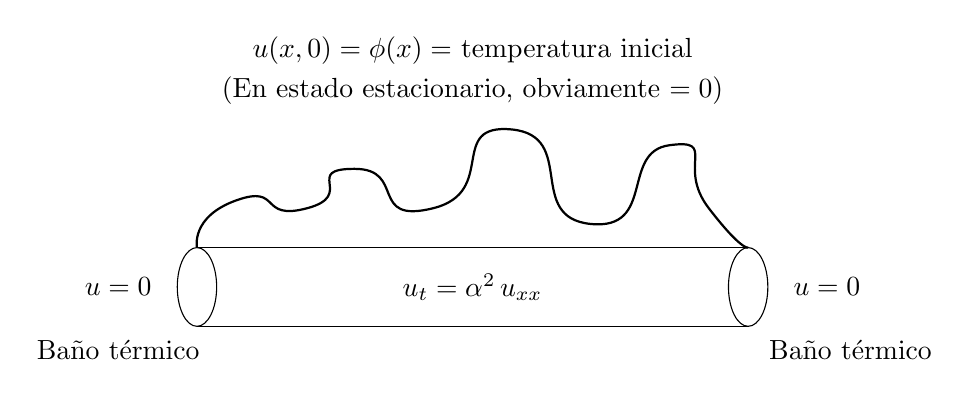
\begin{tikzpicture}
    \draw (0, 0) -- (7, 0);
    \draw (0, 1) -- (7, 1);
    \draw (0, 0.5) ellipse (0.25cm and 0.5 cm);
    \draw (7, 0.5) ellipse (0.25cm and 0.5 cm);
    \node at (3.5, 0.5) {$u_{t} = \alpha^{2} \, u_{xx}$};
    \node at (-1, 0.5) {$u = 0$};
    \node at (-1, -0.3) {Baño térmico};
    \node at (8, 0.5) {$u = 0$};
    \node at (8.3, -0.3) {Baño térmico};
    \draw[thick] plot [smooth,tension=1.5] coordinates{ (0, 1) (0.5, 1.6) (1.4, 1.5) (2, 2) (3, 1.5) (4, 2.5) (5, 1.3) (6, 2.3) (6.5, 1.5) (7, 1)};
    \node at (3.5, 3.5) {$u(x, 0) = \phi(x) = $ temperatura inicial};
    \node at (3.5, 3) {(En estado estacionario, obviamente $=0$)};
\end{tikzpicture}
\end{document}